\documentclass[a4paper,12pt]{article}
\usepackage{ufpb-relatorio}
\usepackage{booktabs}
\usepackage{float}
\usepackage{graphicx}
\usepackage{enumitem}
\addbibresource{references.bib}

% ---------- Metadados da capa ----------
\disciplina{Métodos de Projeto de Software}
\title{Documento de Requisitos}
\subtitulo{CliniCore}
\autor{Beatriz Montenegro Maia Chaves}{20230012233}
\autor{Frankley Kaiky M. Silva}{20220060460}
\autor{Pedro Luca Vaz Matias}{20230089874}
\professor{Raoni Kulesza}
\date{Outubro, 2026}
% Opcionais — valores padrão definidos em ufpb-relatorio.sty:
% \universidade{Universidade Federal da Paraíba}
% \centro{Centro de Informática}
% \local{João Pessoa -- PB}
% \logo{images/logo-ci.jpeg}

\begin{document}

\maketitle

% Importa o Resumo e o Histórico
\section*{Histórico de Revisões}
\begin{table}[H]
  \centering
  \begin{tabular}{|p{2.5cm}|p{1.5cm}|p{7cm}|p{4cm}|}
    \hline
    \textbf{Data} & \textbf{Versão} & \textbf{Descrição} & \textbf{Autor(es)} \\
    \hline
    01/01/2026 & 1.0 & Criação e especificação inicial do documento de requisitos & Beatriz, Pedro e Frankley \\
    \hline
  \end{tabular}
\end{table}

\newpage
\renewcommand{\contentsname}{Sumário}
\tableofcontents
\newpage

% Importa as secções do documento
\section{Introdução}
\label{sec:introducao}

\subsection{Propósito do documento}
O propósito deste documento é especificar os requisitos para o desenvolvimento de um sistema de CRM (Customer/Clinic Relationship Management) voltado para o ambiente de clínicas médicas. O sistema visa gerenciar o relacionamento com os pacientes, possibilitando o agendamento, o acompanhamento de consultas e a comunicação. Um diferencial fundamental deste projeto é a adoção do padrão HL7 FHIR para modelagem e interoperabilidade dos dados de saúde, permitindo comunicação padronizada com sistemas externos.

\subsection{Visão geral do documento}
Esta introdução fornece as informações necessárias para fazer um bom uso deste documento, explicitando seus objetivos e as convenções que foram adotadas no texto, além de conter uma lista de referências para outros documentos relacionados. As demais seções apresentam a especificação do sistema CliniCore e estão organizadas como descrito abaixo.

\begin{itemize}
    \item \textbf{Seção 2 -- Descrição geral do sistema:} apresenta uma visão geral do sistema, caracterizando qual é o seu escopo e descrevendo seus usuários.
    \item \textbf{Seção 3 -- Glossário:} apresenta a definição de termos específicos.
    \item \textbf{Seção 4 -- Elicitação de Requisitos:} descreve as técnicas utilizadas para o levantamento dos dados.
    \item \textbf{Seção 5 -- Análise de Requisitos:} especifica todos os requisitos funcionais e não funcionais do sistema, categorizando usabilidade, segurança, interoperabilidade, entre outros.
    \item \textbf{Seção 6 -- Especificação de Requisitos (casos de uso):} descreve os fluxos de eventos, prioridades, atores, entradas e saídas dos casos de uso mais críticos.
    \item \textbf{Seção 7 -- Análise de casos de uso:} especifica as entidades e o mapeamento dos recursos FHIR adotados.
    \item \textbf{Seção 8 -- Descrição da interface com o usuário:} apresenta especificações para os rascunhos de telas do sistema.
    \item \textbf{Seção 9 -- Diagramas de Arquitetura:} apresenta o modelo arquitetural lógico e de interoperabilidade adotado.
\end{itemize}

\subsection{Documentos relacionados}
Documentos relacionados ao CliniCore e/ou mencionados nas seções a seguir:
\begin{enumerate}[label=\arabic*.]
    \item Especificação Oficial HL7 FHIR (Release 4); 2019; Health Level Seven International;
    \item Lei Geral de Proteção de Dados Pessoais (LGPD) - Lei nº 13.709; 2018; Presidência da República do Brasil;
\end{enumerate}
\newpage
\section{Descrição geral}

\subsection{Motivação}
A gestão do relacionamento com pacientes em clínicas médicas frequentemente sofre com dados fragmentados, ausência de históricos de comunicação unificados e com faltas constantes em consultas. Diante disso, a motivação principal para o desenvolvimento desse sistema é construir uma plataforma centralizada e amigável que otimize o atendimento, aproxime o vínculo da clínica com o paciente e, obrigatoriamente, adote padrões internacionais (FHIR) para permitir fácil integração com outras redes de atenção à saúde.

\subsection{Problemas identificados}
Foram identificados os seguintes problemas:
\begin{itemize}
    \item Dificuldade de rastrear o histórico de interações administrativas com o paciente;
    \item Alta taxa de faltas por deficiência na comunicação e notificação;
    \item Sistemas isolados que não conversam com prontuários externos ou operadoras de saúde;
    \item Incapacidade de gerar visões unificadas sobre a saúde e o engajamento do paciente.
\end{itemize}

\subsection{Visão geral do sistema}
O sistema será um CRM clínico destinado ao gerenciamento do relacionamento entre a clínica e seus pacientes, centralizando informações relevantes para o atendimento e para a gestão da clínica. As principais funcionalidades inicialmente previstas são o cadastro padronizado de pacientes e profissionais de saúde, o agendamento e gerenciamento da agenda da clínica, o registro do histórico de comunicações e o envio de notificações e lembretes. O sistema também permitirá o registro de encontros clínicos e de observações em alto nível, além de possibilitar a interoperabilidade com outros sistemas de saúde por meio da exposição e do consumo de recursos padronizados pelo FHIR (Fast Healthcare Interoperability Resources).

Entretanto, como parte do escopo negativo, o sistema não terá como objetivo atuar como um Prontuário Eletrônico do Paciente (PEP/EHR) de alta complexidade ou como um sistema de gestão hospitalar. Dessa forma, funcionalidades como prescrição eletrônica avançada, gestão de leitos, faturamento hospitalar e integração com equipamentos de diagnóstico por imagem não serão feitas.

\subsection{Usuários do sistema}
Os usuários previstos são:
\begin{itemize}
    \item \textbf{Administrador/Gestor da Clínica:} Responsável pelas configurações globais, gestão da organização (clínica) e extração de relatórios de engajamento e faltas.
    \item \textbf{Recepcionista/Secretário:} Usuário de linha de frente que opera o sistema para gerenciar filas, agendamentos, contatos e o cadastro demográfico dos pacientes.
    \item \textbf{Profissional de Saúde:} Usuário que visualiza a agenda diária e registra informações básicas do encontro clínico de modo simplificado.
    \item \textbf{Paciente:} Usuário externo que pode acessar um portal ou interagir passivamente através de notificações e lembretes para confirmação de agendamentos.
\end{itemize}

\subsection{Suposições e restrições gerais}
\begin{itemize}
    \item A arquitetura deve obrigatoriamente mapear e comunicar dados respeitando o padrão HL7 FHIR.
    \item Como o sistema trata de dados sensíveis de saúde, a conformidade com as exigências de privacidade e proteção da LGPD é mandatória.
    \item O sistema dependerá de conectividade com a internet para sua operação e para comunicação com APIs externas.
\end{itemize}
\newpage
\section{Glossário}
\begin{itemize}
    \item \textbf{Agendamento:} Ação de reservar um bloco de tempo (Slot) na agenda de um profissional de saúde para o atendimento de um paciente específico.
    \item \textbf{Atendimento:} O evento no qual a interação direta entre o Paciente e o Profissional de Saúde de fato ocorre, sendo o momento onde as observações e diagnósticos básicos são registrados no sistema.
    \item \textbf{CRM (Customer Relationship Management):} Refere-se à plataforma voltada para o gerenciamento do relacionamento com o paciente, focando no histórico de contatos, otimização da agenda, comunicação de lembretes e retenção.
    \item \textbf{FHIR (Fast Healthcare Interoperability Resources):} Padrão desenvolvido pelo HL7 para troca eletrônica de informações de saúde.
    \item \textbf{LGPD (Lei Geral de Proteção de Dados):} Legislação brasileira que regula o tratamento de dados pessoais.
    \item \textbf{Paciente:} Indivíduo cadastrado na clínica que recebe ou está agendado para receber cuidados médicos ou administrativos. É a entidade central em torno da qual o CRM opera.
    \item \textbf{Profissional de Saúde:} Colaborador da clínica autorizado a realizar os atendimentos clínicos, visualizar as agendas de consultas e registrar anotações no histórico de saúde do paciente.
\end{itemize}
\newpage
\section{Elicitação de Requisitos}

\subsection{Reunião de grupo}
Foi utilizada uma discussão colaborativa entre os integrantes do grupo por mensagens no WhatsApp. A coleta ocorreu principalmente entre 29/09/2026, às 18:34, e 30/09/2026, às 18:58, em ambiente remoto. Participaram Pedro Luca Vaz Matias, Beatriz Montenegro e Frankley Kaiky M. Silva. A técnica foi escolhida porque o projeto ainda estava na fase de definição do tema e os integrantes precisavam alinhar a necessidade atendida, os atores e os riscos iniciais.

Como resultados, o grupo definiu:
\begin{itemize}
    \item O escopo principal do sistema, focando em um CRM ambulatorial (CliniCore) para gestão de relacionamento e agendamentos, descartando a complexidade de um prontuário eletrônico hospitalar completo.
    \item Os atores principais que interagem com o sistema: Administrador da Clínica, Recepcionista, Profissional de Saúde e Paciente.
    \item A necessidade de uma interface de interoperabilidade baseada no padrão HL7 FHIR.
\end{itemize}

\subsection{Análise Documental e Benchmarking}
Esta técnica consistiu na pesquisa de documentações técnicas e na avaliação de funcionalidades presentes em sistemas de gestão de clínicas já estabelecidos no mercado. A coleta ocorreu de forma assíncrona entre 30/09/2026 e 01/10/2026, em ambiente remoto, conduzida pelos mesmos integrantes do grupo. A técnica foi escolhida por ser altamente viável na ausência de stakeholders reais, permitindo que a equipe compreendesse os fluxos de trabalho padrão de uma clínica médica e os requisitos técnicos de interoperabilidade sem depender do contato direto com usuários finais.

\subsection{Considerações Finais}
A elicitação confirmou a necessidade de um sistema que separe a complexidade de um PEP robusto da agilidade exigida para a gestão do relacionamento e da agenda, enfatizando a necessidade de uma base de dados que seja facilmente interpretável por outros sistemas usando FHIR.
\newpage
\section{Análise de Requisitos}

\subsection{Requisitos funcionais}
\begin{table}[H]
  \centering
  \small
  \begin{tabular}{|p{1cm}|p{3.5cm}|p{5cm}|p{2cm}|p{2cm}|}
    \hline
    \textbf{ID} & \textbf{Nome} & \textbf{Descrição} & \textbf{Casos de Uso} & \textbf{Prioridade} \\
    \hline
    RF01 & Cadastrar Paciente & O sistema deve permitir o cadastro, edição e inativação de pacientes, registrando dados demográficos, identificadores únicos (como CPF) e informações de contato. & UC01 & Essencial \\
    \hline
    RF02 & Gerenciar Profissionais e Clínica & O sistema deve manter o cadastro da organização (clínica), dos profissionais de saúde e seus respectivos papéis e especialidades. & UC01, UC02, UC03 & Essencial \\
    \hline
    RF03 & Agendar Consulta & O sistema deve permitir o agendamento, cancelamento e reagendamento de consultas com base na disponibilidade (agenda) dos profissionais. & UC02 & Essencial \\
    \hline
    RF04 & Registrar Atendimento e Interações Clínicas & O profissional de saúde deve ser capaz de registrar o início e fim de um encontro clínico presencial ou remoto, documentando informações básicas do atendimento e possíveis diagnósticos ou observações. & UC03 & Essencial \\
    \hline
    RF05 & Gerenciar Comunicações e Lembretes & O sistema deve registrar todas as interações com o paciente (ligações, e-mails, mensagens) e enviar solicitações de confirmação de agendamento automatizadas. & UC02 & Essencial \\
    \hline
    RF06 & Controle de Acesso e Perfil de Usuário & O sistema deve garantir que o acesso aos dados dos pacientes seja restrito aos usuários autenticados e de acordo com seus respectivos papéis de acesso (Recepcionista vs. Médico) & UC01, UC02, UC03 & Essencial \\
    \hline
  \end{tabular}
\end{table}

\subsection{Requisitos não funcionais}
\begin{table}[H]
  \centering
  \small
  \begin{tabular}{|p{1cm}|p{3cm}|p{3cm}|p{5cm}|p{2cm}|}
    \hline
    \textbf{ID} & \textbf{Categoria} & \textbf{Nome} & \textbf{Descrição} & \textbf{Prioridade} \\
    \hline
    NF01 & Usabilidade & Interface Intuitiva e Responsiva & A interface do usuário deve ser intuitiva e fácil de usar, logo, o usuário não pode demorar mais do que 10 segundos para encontrar qualquer operação do sistema & Essencial \\
    \hline
    NF02 & Segurança & Autenticação e Autorização & O acesso à plataforma exige autenticação por senha forte e controle de autorização baseado em papéis (RBAC - Role-Based Access Control) seguindo o princípio do menor privilégio. & Essencial \\
    \hline
    NF03 & Segurança & Criptografia de Dados & Todo o tráfego de dados entre a aplicação, o backend e APIs externas deve obrigatoriamente utilizar o protocolo HTTPS (TLS 1.2+) & Essencial \\
    \hline
    NF04 & Desempenho & Tempo de Resposta & O sistema deve retornar os resultados das buscas por pacientes e disponibilização de horários de agenda em no máximo 2 segundos para manter o fluxo rápido. & Importante \\
    \hline
    NF05 & Privacidade & Adequação à LGPD & O sistema deve tratar dados de saúde de forma segura, exigindo base legal, consentimento quando aplicável e permitindo a pseudo-anonimização em bases analíticas. & Essencial \\
    \hline
    NF06 & Interoperabilidade & Adoção do Padrão FHIR & O sistema deve suportar a serialização/deserialização de dados demográficos e agendamentos no formato JSON em estrita conformidade com a estrutura dos recursos do HL7 FHIR & Essencial \\
    \hline
  \end{tabular}
\end{table}
\newpage
\section{Especificação de Requisitos}

\subsection{Descrição de Casos de Uso}

\subsubsection{Cadastrar Paciente}
\begin{table}[H]
  \centering
  \begin{tabular}{|p{4cm}|p{11cm}|}
    \hline
    \textbf{Identificador} & UC01 \\ \hline
    \textbf{Importância} & Essencial \\ \hline
    \textbf{Sumário} & Permite criar um novo registro no sistema representando um indivíduo que receberá cuidados na clínica. \\ \hline
    \textbf{Atores} & Recepcionista \\ \hline
    \textbf{Pré-condições} & O ator deve estar autenticado e o paciente deve fornecer dados válidos de identificação e contato. \\ \hline
    \textbf{Fluxo principal} & 
    1. O ator acessa a tela de cadastro.\newline
    2. O sistema exibe o formulário de cadastro.\newline
    3. O ator preenche os dados demográficos e contatos.\newline
    4. O ator solicita salvar os dados.\newline
    5. O sistema valida as informações.\newline
    6. O sistema registra o cadastro e vincula um identificador único.\newline
    7. O sistema informa o sucesso da operação. \\ \hline
    \textbf{Fluxos de exceção} & 
    - FE1: Se os dados forem inválidos, o sistema informa os campos com inconsistência e volta para o passo 3.\newline
    - FE2: O CPF já está vinculado, o sistema informa a duplicidade e oferece atalho para o perfil. \\ \hline
    \textbf{Pós-condição} & Um novo registro de paciente é salvo no banco de dados. O paciente fica disponível para agendamentos. \\ \hline
  \end{tabular}
\end{table}

\subsubsection{Agendar Consulta}
\begin{table}[H]
  \centering
  \begin{tabular}{|p{4cm}|p{11cm}|}
    \hline
    \textbf{Identificador} & UC02 \\ \hline
    \textbf{Importância} & Essencial \\ \hline
    \textbf{Sumário} & Permite definir uma reserva de tempo entre o paciente, o profissional e a clínica. \\ \hline
    \textbf{Atores} & Recepcionista, Paciente \\ \hline
    \textbf{Pré-condições} & O paciente deve existir no sistema e o profissional deve ter horários de agenda disponíveis. \\ \hline
    \textbf{Fluxo principal} & 
    1. O ator seleciona um Paciente na base de dados.\newline
    2. O ator escolhe a opção ``Agendar Consulta''.\newline
    3. O ator escolhe a especialidade e o profissional de Saúde.\newline
    4. O sistema consulta a Grade de Agenda (Schedule).\newline
    5. O sistema lista os horários disponíveis (Slot).\newline
    6. O ator seleciona data e horário.\newline
    7. O ator confirma o agendamento.\newline
    8. O sistema atualiza o status da agenda e salva a consulta.\newline
    9. O sistema agenda o disparo de um lembrete automático. \\ \hline
    \textbf{Fluxos de exceção} & 
    - FE1: O ator busca uma consulta existente e altera apenas o Slot de tempo para reagendamento. O sistema cancela o slot anterior e ocupa o novo. \\ \hline
    \textbf{Pós-condição} & Uma consulta é gerada com status ``agendado'' e um lembrete é engatilhado. \\ \hline
  \end{tabular}
\end{table}

\subsubsection{Registrar Atendimento Básico}
\begin{table}[H]
  \centering
  \begin{tabular}{|p{4cm}|p{11cm}|}
    \hline
    \textbf{Identificador} & UC03 \\ \hline
    \textbf{Importância} & Essencial \\ \hline
    \textbf{Sumário} & Permite que o profissional registre que a consulta ocorreu, suas observações e finalização. \\ \hline
    \textbf{Atores} & Profissional de saúde \\ \hline
    \textbf{Pré-condições} & O ator deve estar autenticado. Uma consulta deve existir para o dia corrente com status ``aguardando atendimento''. \\ \hline
    \textbf{Fluxo principal} & 
    1. O ator visualiza a fila de pacientes do dia.\newline
    2. O ator seleciona o paciente em espera e inicia o atendimento.\newline
    3. O sistema vincula o status do agendamento para ``em andamento''.\newline
    4. O ator documenta o motivo da visita, o histórico atual e aferições básicas.\newline
    5. O ator adiciona possíveis condições ou diagnósticos.\newline
    6. O ator encerra o atendimento.\newline
    7. O sistema altera o status do encontro para ``finalizado'' e salva no histórico geral. \\ \hline
    \textbf{Pós-condição} & O encontro clínico é salvo com status ``finalizado''. Possíveis problemas ou anotações ficam registrados no histórico do paciente. \\ \hline
  \end{tabular}
\end{table}

\subsection{Diagrama Casos de Uso}
Considerando os usuários do sistema, que foram identificados como os atores, e os requisitos documentados anteriormente, foi possível definir o diagrama de caso de uso (Figura~\ref{fig:diagrama_uc}), ilustrando as diversas interações que os usuários terão com o sistema.

\begin{figure}[H]
  \centering
  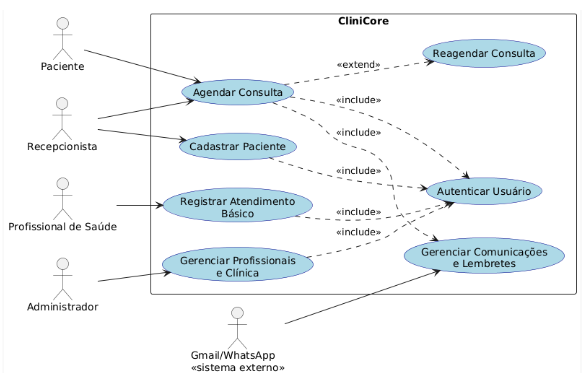
\includegraphics[width=0.9\textwidth]{images/diagrama-casos-de-uso.png}
  \caption{Diagrama de Casos de Uso do CliniCore.}
  \label{fig:diagrama_uc}
\end{figure}
\newpage
\section{Análise de casos de uso (diagrama de classes de análise)}
O diagrama de classes de análise apresenta a estrutura conceitual do domínio do sistema, detalhando as entidades principais e as associações entre elas. Este modelo destaca o alinhamento estrutural do CRM com o padrão de interoperabilidade HL7 FHIR.

\begin{figure}[H]
  \centering
  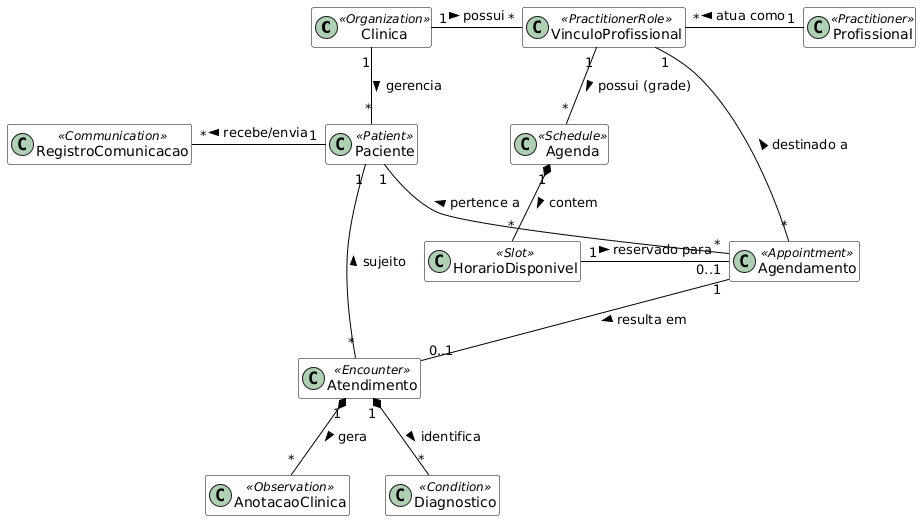
\includegraphics[width=\textwidth]{images/diagrama-classes-de-analise.png}
  \caption{Diagrama de classes de análise.}
  \label{fig:diagrama_classes}
\end{figure}
\newpage
\section{Descrição da interface com o usuário}
Esta seção apresenta os protótipos de interface (mockups) para o sistema CliniCore, com o objetivo de tangibilizar os requisitos funcionais descritos nas seções anteriores. Elas possuem caráter ilustrativo, servindo para facilitar a compreensão da disposição das informações, da ergonomia e do fluxo de navegação idealizado para a aplicação.

\begin{figure}[H]
  \centering
  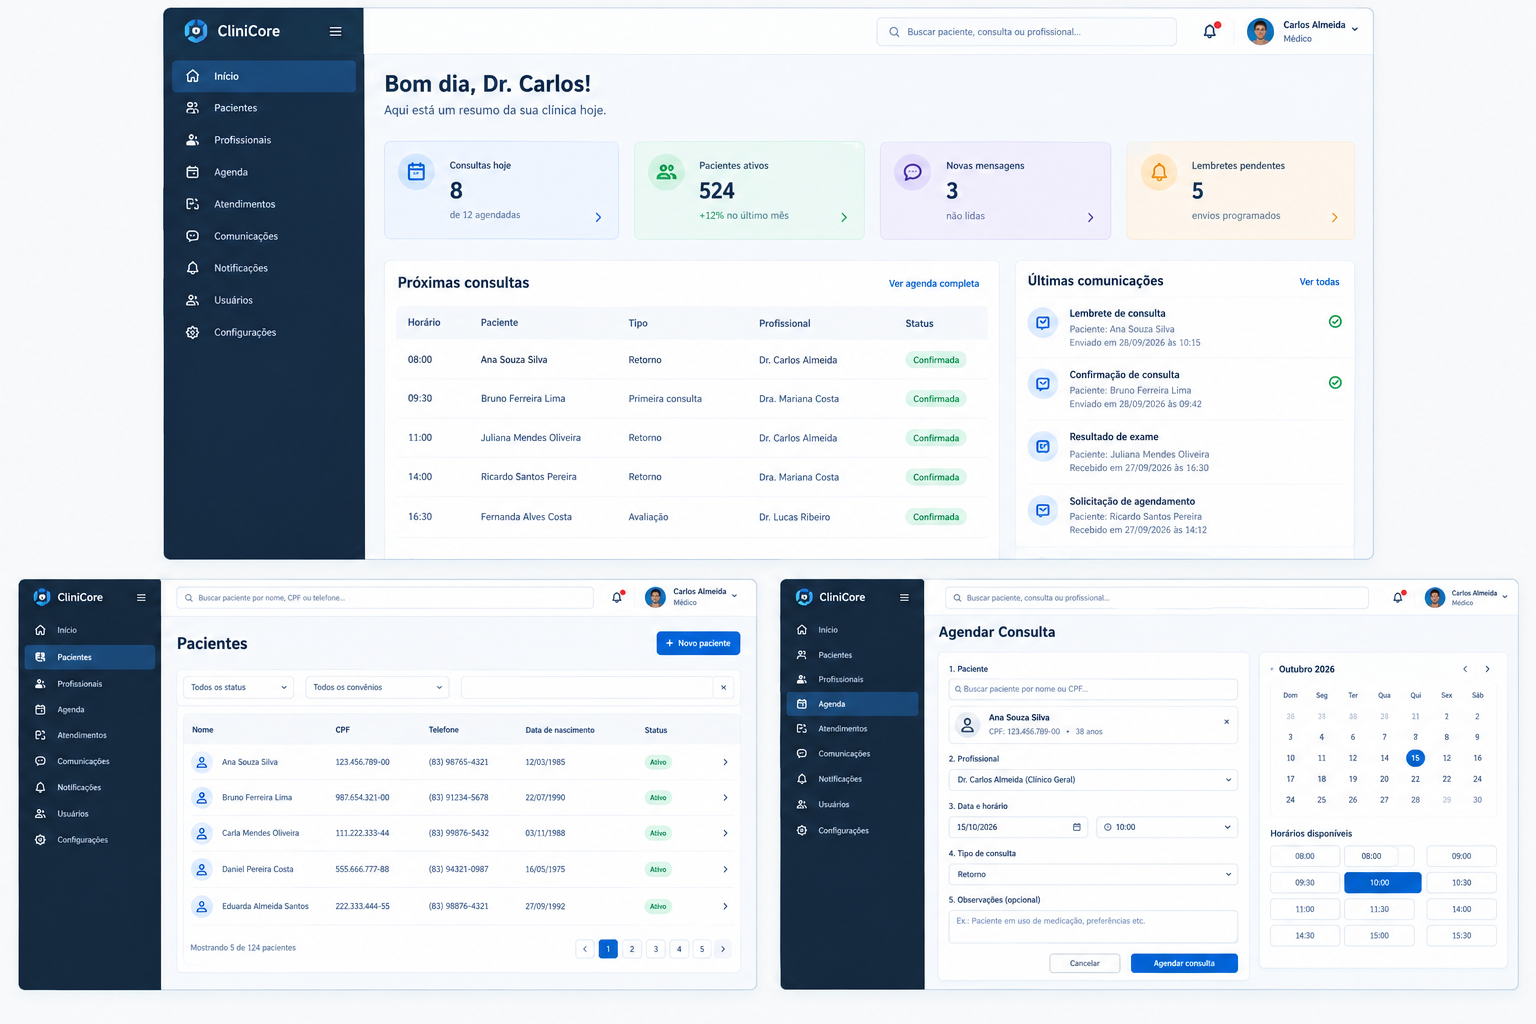
\includegraphics[width=\textwidth]{images/mockups-interface.png}
  \caption{Protótipos da interface do sistema CliniCore.}
  \label{fig:mockups}
\end{figure}
\newpage
\section{Diagramas de Arquitetura}
O diagrama de arquitetura detalha a organização lógica e tecnológica do sistema sob um modelo de camadas. A representação evidencia a separação entre a interface de usuário (Frontend SPA), a API central baseada em Node.js com Express, os serviços de persistência de dados e, fundamentalmente, a camada de interoperabilidade (FHIR Facade). Esta última atua como o componente responsável por mediar a comunicação segura e padronizada com sistemas externos de saúde.

\begin{figure}[H]
  \centering
  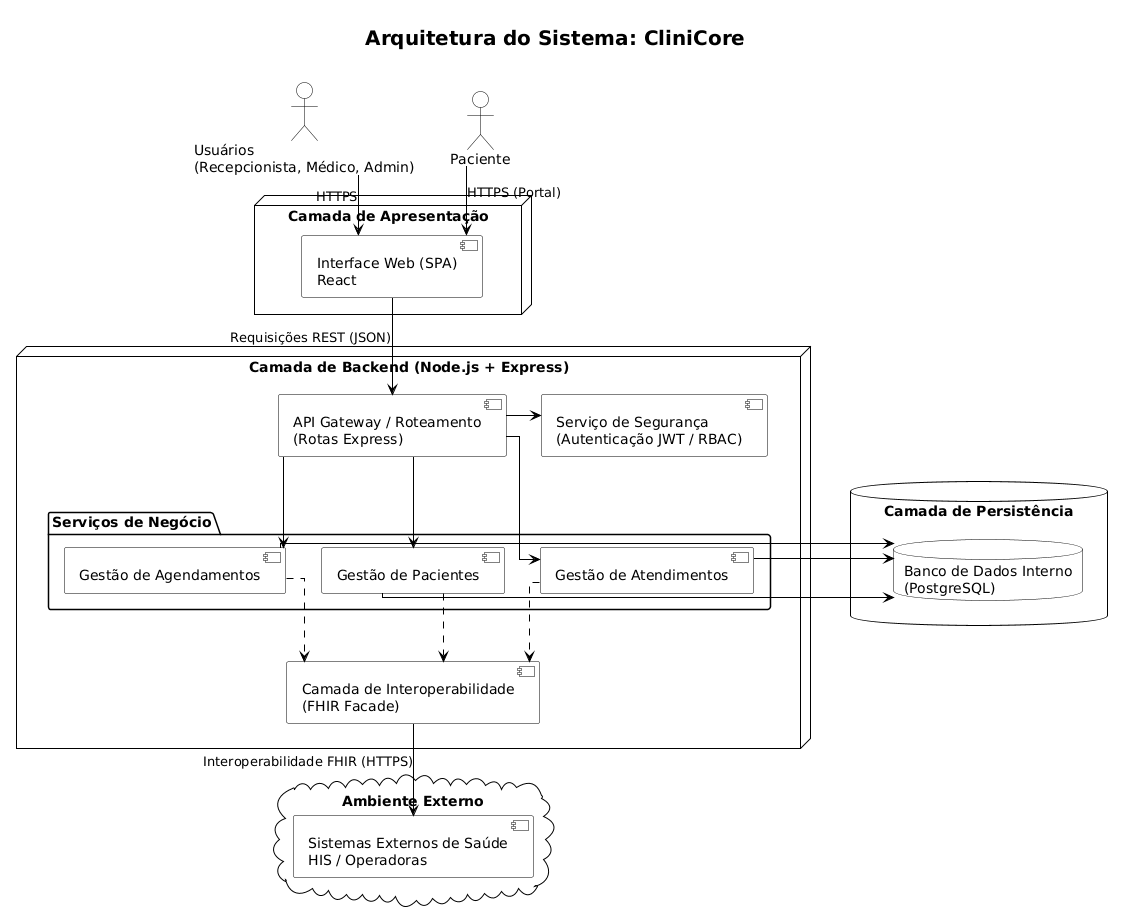
\includegraphics[width=\textwidth]{images/diagrama-arquitetura.png}
  \caption{Diagrama de Arquitetura do CliniCore.}
  \label{fig:arquitetura}
\end{figure}


\end{document}